%========================================
% LESSON CONTENT: Funciones
%========================================

\lesson{Funciones — Definición y gráficas}

\noindent\textbf{Temario:}
\begin{itemize}[itemsep=0pt]
    \item Definición de función
    \item Notación funcional y evaluación
    \item Dominio y rango
    \item Prueba de la recta vertical
    \item Gráficas de funciones simples
\end{itemize}

\vspace{0.3cm}
\noindent\textit{Nota:} Una función asigna a cada elemento del dominio \textbf{exactamente un} elemento del rango.

%========================================
\subsectiontitle{Definición de función}
%========================================

\begin{definition}
Una \textbf{función} es una relación entre dos conjuntos en la que a cada elemento del primer conjunto (dominio) le corresponde \textbf{exactamente un} elemento del segundo conjunto (rango).

\vspace{0.3cm}
\noindent\textbf{Elementos clave:}
\begin{itemize}[itemsep=2pt]
    \item \textbf{Dominio:} Conjunto de valores de entrada permitidos (usualmente $x$)
    \item \textbf{Rango:} Conjunto de valores de salida posibles (usualmente $y$ o $f(x)$)
    \item \textbf{Notación funcional:} $f(x)$ se lee ``f de x''
\end{itemize}
\end{definition}

\begin{center}
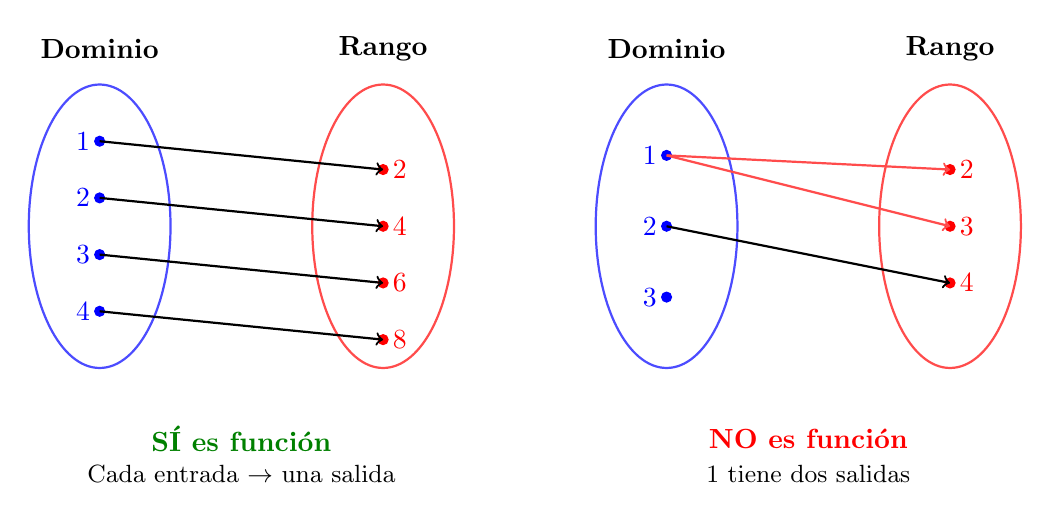
\begin{tikzpicture}[scale=0.9]
    % Function example (left)
    \begin{scope}[xshift=0cm]
        \draw[thick, blue!70] (0,0) ellipse (1cm and 2cm);
        \draw[thick, red!70] (4,0) ellipse (1cm and 2cm);
        \node at (0,2.5) {\textbf{Dominio}};
        \node at (4,2.5) {\textbf{Rango}};

        % Points in domain
        \filldraw[blue] (0,1.2) circle (2pt) node[left] {$1$};
        \filldraw[blue] (0,0.4) circle (2pt) node[left] {$2$};
        \filldraw[blue] (0,-0.4) circle (2pt) node[left] {$3$};
        \filldraw[blue] (0,-1.2) circle (2pt) node[left] {$4$};

        % Points in range
        \filldraw[red] (4,0.8) circle (2pt) node[right] {$2$};
        \filldraw[red] (4,0) circle (2pt) node[right] {$4$};
        \filldraw[red] (4,-0.8) circle (2pt) node[right] {$6$};
        \filldraw[red] (4,-1.6) circle (2pt) node[right] {$8$};

        % Arrows
        \draw[->, thick] (0,1.2) -- (4,0.8);
        \draw[->, thick] (0,0.4) -- (4,0);
        \draw[->, thick] (0,-0.4) -- (4,-0.8);
        \draw[->, thick] (0,-1.2) -- (4,-1.6);

        \node at (2,-3) {\textcolor{green!50!black}{\textbf{SÍ es función}}};
        \node at (2,-3.5) {\small Cada entrada $\to$ una salida};
    \end{scope}

    % Non-function example (right)
    \begin{scope}[xshift=8cm]
        \draw[thick, blue!70] (0,0) ellipse (1cm and 2cm);
        \draw[thick, red!70] (4,0) ellipse (1cm and 2cm);
        \node at (0,2.5) {\textbf{Dominio}};
        \node at (4,2.5) {\textbf{Rango}};

        % Points in domain
        \filldraw[blue] (0,1) circle (2pt) node[left] {$1$};
        \filldraw[blue] (0,0) circle (2pt) node[left] {$2$};
        \filldraw[blue] (0,-1) circle (2pt) node[left] {$3$};

        % Points in range
        \filldraw[red] (4,0.8) circle (2pt) node[right] {$2$};
        \filldraw[red] (4,0) circle (2pt) node[right] {$3$};
        \filldraw[red] (4,-0.8) circle (2pt) node[right] {$4$};

        % Arrows (1 maps to two values!)
        \draw[->, thick, red!70] (0,1) -- (4,0.8);
        \draw[->, thick, red!70] (0,1) -- (4,0);
        \draw[->, thick] (0,0) -- (4,-0.8);

        \node at (2,-3) {\textcolor{red}{\textbf{NO es función}}};
        \node at (2,-3.5) {\small 1 tiene dos salidas};
    \end{scope}
\end{tikzpicture}
\end{center}

\begin{example}
Determine si la relación es función:
\begin{enumerate}[label=\textbf{\alph*.}]
    \item $\{(1,2), (2,4), (3,6), (4,8)\}$ \quad \textcolor{green!50!black}{$\checkmark$ Sí es función}
    \item $\{(1,2), (1,3), (2,4)\}$ \quad \textcolor{red}{$\times$ No es función (1 tiene dos salidas)}
\end{enumerate}
\end{example}

%========================================
\subsectiontitle{Notación funcional y evaluación}
%========================================

\noindent\textbf{Procedimiento:} Para evaluar $f(a)$, sustituya $x=a$ en la expresión de $f(x)$ y simplifique.

\begin{example}
Dada $f(x) = x^2 - 3x + 1$, evalúe:

\noindent\textbf{a)} $f(4)$

\solution
\begin{align*}
f(4) &= (4)^2 - 3(4) + 1\\
&= 16 - 12 + 1\\
&= 5
\end{align*}

\noindent\textbf{b)} $f(a+1)$

\solution
\begin{align*}
f(a+1) &= (a+1)^2 - 3(a+1) + 1\\
&= a^2 + 2a + 1 - 3a - 3 + 1\\
&= a^2 - a - 1
\end{align*}
\end{example}

\begin{warning}
Al sustituir expresiones, use \textbf{paréntesis}:
$$f(a+1) \ne a+1^2 - 3(a+1) + 1$$
$$f(a+1) = (a+1)^2 - 3(a+1) + 1 \quad \checkmark$$
\end{warning}

%========================================
\subsectiontitle{Dominio y rango}
%========================================

\noindent\textbf{Restricciones comunes:}
\begin{itemize}[itemsep=2pt]
    \item \textbf{División:} El denominador $\ne 0$
    \item \textbf{Raíces pares:} El radicando $\ge 0$
    \item \textbf{Funciones lineales:} Dominio siempre $(-\infty, \infty)$
\end{itemize}

\begin{example}
Encuentre el dominio:

\noindent\textbf{a)} $f(x) = \dfrac{1}{x-3}$

\solution El denominador no puede ser cero: $x - 3 \ne 0 \Rightarrow x \ne 3$

\textbf{Dominio:} $(-\infty, 3) \cup (3, \infty)$

\vspace{0.3cm}
\noindent\textbf{b)} $g(x) = \sqrt{2x-6}$

\solution Necesitamos $2x - 6 \ge 0$:
\begin{align*}
2x &\ge 6\\
x &\ge 3
\end{align*}

\textbf{Dominio:} $[3, \infty)$

\vspace{0.3cm}
\noindent\textbf{c)} $h(x) = \dfrac{\sqrt{x+1}}{x-2}$

\solution Necesitamos $x + 1 \ge 0$ (radical) y $x - 2 \ne 0$ (denominador):
\begin{itemize}[itemsep=2pt]
    \item $x \ge -1$
    \item $x \ne 2$
\end{itemize}

\textbf{Dominio:} $[-1, 2) \cup (2, \infty)$
\end{example}

\newpage
%========================================
\subsectiontitle{Prueba de la recta vertical}
%========================================

\begin{theorem}
\textbf{Prueba de la recta vertical:} Una gráfica representa una función si y solo si \textbf{ninguna recta vertical} interseca la gráfica en más de un punto.
\end{theorem}

\begin{center}
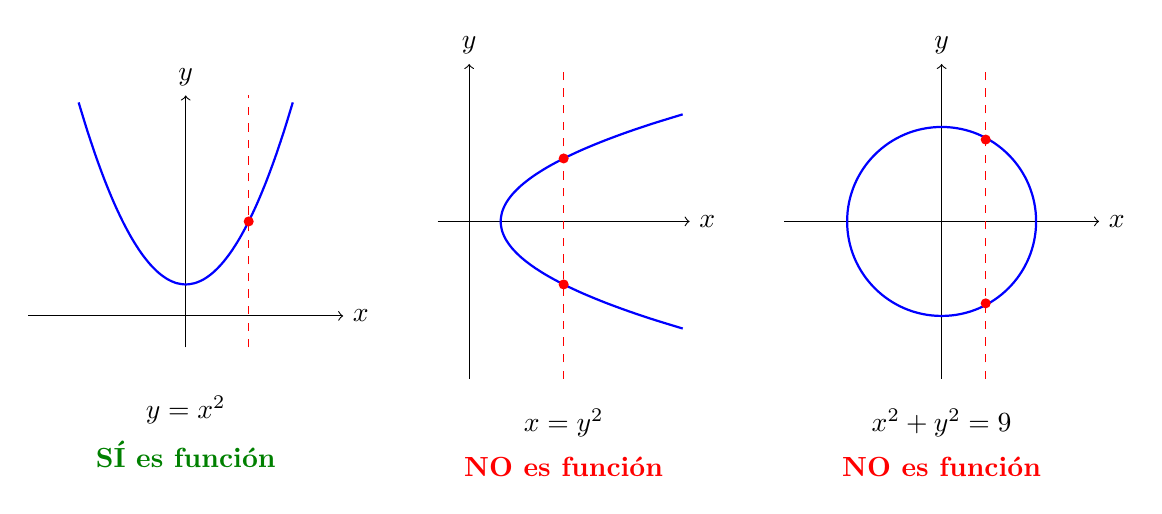
\begin{tikzpicture}[scale=0.8]
    % Example 1: Parabola (is a function)
    \begin{scope}[xshift=0cm, yshift=-1.5cm]
        \draw[->] (-2.5,0) -- (2.5,0) node[right] {$x$};
        \draw[->] (0,-0.5) -- (0,3.5) node[above] {$y$};
        \draw[domain=-1.7:1.7, smooth, blue, thick] plot (\x, {\x*\x + 0.5});

        % Vertical line test
        \draw[dashed, red] (1,-0.5) -- (1,3.5);
        \filldraw[red] (1,1.5) circle (2pt);

        \node at (0,-1.5) {$y = x^2$};
        \node[green!50!black] at (0,-2.2) {\textbf{SÍ es función}};
    \end{scope}

    % Example 2: Horizontal parabola (NOT a function)
    \begin{scope}[xshift=4.5cm]
        \draw[->] (-0.5,0) -- (3.5,0) node[right] {$x$};
        \draw[->] (0,-2.5) -- (0,2.5) node[above] {$y$};
        \draw[domain=-1.7:1.7, smooth, blue, thick] plot ({\x*\x + 0.5}, \x);

        % Vertical line test
        \draw[dashed, red] (1.5,-2.5) -- (1.5,2.5);
        \filldraw[red] (1.5,1) circle (2pt);
        \filldraw[red] (1.5,-1) circle (2pt);

        \node at (1.5,-3.2) {$x = y^2$};
        \node[red] at (1.5,-3.9) {\textbf{NO es función}};
    \end{scope}

    % Example 3: Circle (NOT a function)
    \begin{scope}[xshift=12cm]
        \draw[->] (-2.5,0) -- (2.5,0) node[right] {$x$};
        \draw[->] (0,-2.5) -- (0,2.5) node[above] {$y$};
        \draw[blue, thick] (0,0) circle (1.5cm);

        % Vertical line test
        \draw[dashed, red] (0.7,-2.5) -- (0.7,2.5);
        \filldraw[red] (0.7,1.3) circle (2pt);
        \filldraw[red] (0.7,-1.3) circle (2pt);

        \node at (0,-3.2) {$x^2 + y^2 = 9$};
        \node[red] at (0,-3.9) {\textbf{NO es función}};
    \end{scope}
\end{tikzpicture}
\end{center}

%========================================
\subsectiontitle{Gráficas de funciones simples}
%========================================

\begin{center}
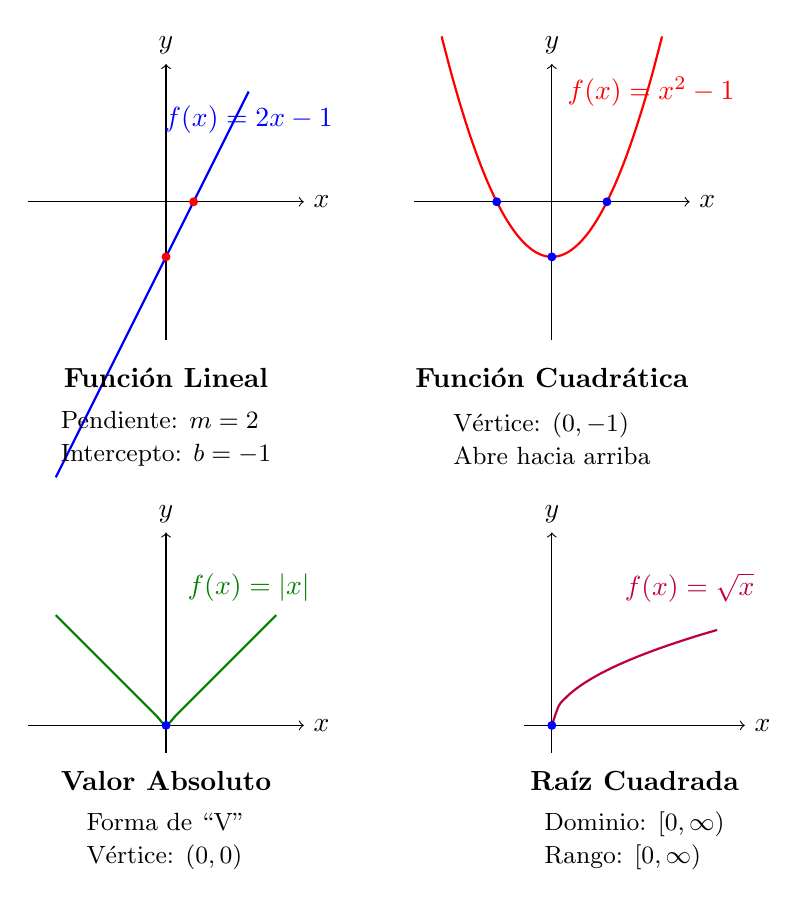
\begin{tikzpicture}[scale=0.7]
    % Linear function
    \begin{scope}[xshift=0cm, yshift=6cm]
        \draw[->] (-2.5,0) -- (2.5,0) node[right] {$x$};
        \draw[->] (0,-2.5) -- (0,2.5) node[above] {$y$};
        \draw[domain=-2:1.5, smooth, blue, thick] plot (\x, {2*\x - 1});

        \node[blue] at (1.5,1.5) {$f(x) = 2x - 1$};
        \node at (0,-3.2) {\textbf{Función Lineal}};
        \node[align=left] at (0,-4.3) {\small Pendiente: $m=2$\\ \small Intercepto: $b=-1$};

        % Mark intercepts
        \filldraw[red] (0,-1) circle (2pt);
        \filldraw[red] (0.5,0) circle (2pt);
    \end{scope}

    % Quadratic function
    \begin{scope}[xshift=7cm, yshift=6cm]
        \draw[->] (-2.5,0) -- (2.5,0) node[right] {$x$};
        \draw[->] (0,-2.5) -- (0,2.5) node[above] {$y$};
        \draw[domain=-2:2, smooth, red, thick] plot (\x, {\x*\x - 1});

        \node[red] at (1.8,2) {$f(x) = x^2 - 1$};
        \node at (0,-3.2) {\textbf{Función Cuadrática}};
        \node[align=left] at (0,-4.3) {\small Vértice: $(0,-1)$\\ \small Abre hacia arriba};

        % Mark vertex and intercepts
        \filldraw[blue] (0,-1) circle (2pt);
        \filldraw[blue] (1,0) circle (2pt);
        \filldraw[blue] (-1,0) circle (2pt);
    \end{scope}

    % Absolute value function
    \begin{scope}[xshift=0cm, yshift=-3.5cm]
        \draw[->] (-2.5,0) -- (2.5,0) node[right] {$x$};
        \draw[->] (0,-0.5) -- (0,3.5) node[above] {$y$};
        \draw[domain=-2:2, smooth, green!50!black, thick] plot (\x, {abs(\x)});

        \node[green!50!black] at (1.5,2.5) {$f(x) = |x|$};
        \node at (0,-1) {\textbf{Valor Absoluto}};
        \node[align=left] at (0,-2.1) {\small Forma de ``V''\\ \small Vértice: $(0,0)$};

        % Mark vertex
        \filldraw[blue] (0,0) circle (2pt);
    \end{scope}

    % Square root function
    \begin{scope}[xshift=7cm, yshift=-3.5cm]
        \draw[->] (-0.5,0) -- (3.5,0) node[right] {$x$};
        \draw[->] (0,-0.5) -- (0,3.5) node[above] {$y$};
        \draw[domain=0:3, smooth, purple, thick] plot (\x, {sqrt(\x)});

        \node[purple] at (2.5,2.5) {$f(x) = \sqrt{x}$};
        \node at (1.5,-1) {\textbf{Raíz Cuadrada}};
        \node[align=left] at (1.5,-2.1) {\small Dominio: $[0,\infty)$\\ \small Rango: $[0,\infty)$};

        % Mark starting point
        \filldraw[blue] (0,0) circle (2pt);
    \end{scope}
\end{tikzpicture}
\end{center}

\vspace{0.5cm}
\begin{center}
\begin{tabular}{|l|c|c|c|}
\hline
\textbf{Función} & \textbf{Forma} & \textbf{Dominio} & \textbf{Rango} \\
\hline
Lineal: $f(x) = mx + b$ & Recta & $(-\infty, \infty)$ & $(-\infty, \infty)$ \\
\hline
Cuadrática: $f(x) = ax^2 + bx + c$ & Parábola & $(-\infty, \infty)$ & Variable \\
\hline
Valor absoluto: $f(x) = |x|$ & V & $(-\infty, \infty)$ & $[0, \infty)$ \\
\hline
Raíz cuadrada: $f(x) = \sqrt{x}$ & Curva & $[0, \infty)$ & $[0, \infty)$ \\
\hline
\end{tabular}
\end{center}

\begin{warning}
\textbf{Errores comunes:}
\begin{itemize}[itemsep=2pt]
    \item Confundir $f(x) = x^2$ (función) con $x = y^2$ (no es función)
    \item No considerar restricciones de dominio al graficar
    \item Olvidar usar paréntesis al evaluar funciones
\end{itemize}
\end{warning}
